\chapter{CLIPS}

Il presente capitolo illustra le principali scelte implementative adottate nella realizzazione di un sistema esperto facendo uso dello strumento \texttt{clips}. Tale sistema ha come scopo aiutare l'utente a scegliere un itinerario per una ipotetica vacanza; nel farlo, deve tenere conto delle preferenze espresse. Deve essere inoltre in grado di fornire una soluzione approssimata anche quando non dispone di informazione completa, ovvero nel caso in cui l'utente scelga di ignorare ad una o più delle domande poste dal sistema.

\section{Organizzazione di moduli e file}

\subsection{Suddivisione dei moduli}

Per ragioni di leggibilità e manutenibilità, il codice è organizzato in moduli. Tra questi ultimi è possibile operare una distinzione logica fra moduli ``di dominio", che definiscono template e fatti con cui si rappresentano le entità (località, hotel, preferenze $\dots$), e moduli ``di reasoning", che definiscono le regole di inferenza grazie alle quali vengono costruiti e valutati i possibili itinerari. 
I moduli di dominio sono di seguito elencati:


\begin{itemize}
\item \textbf{QUESTION}\\
Contiene template e fatti relativi alle domande che il sistema può porre all'utente. Inoltre, memorizza le risposte fornite per renderle disponibili al modulo di reasoning incaricato di fare inferenza basandosi sulle preferenze espresse (\texttt{QUESTION-INFERENCE}).
\item \textbf{RESORT}\\
Contiene template e fatti relativi alle possibili località turistiche, alle loro qualità e ai collegamenti che consentono lo spostamento tra località differenti.
\item \textbf{HOTEL}\\
Contiene template e fatti relativi agli hotel presenti nelle diverse località turistiche.
\item \textbf{TRIP}\\
Contiene i template relativi ai viaggi da proporre all'utente e ai vari aspetti che li caratterizzano, come ad esempio i possibili cammini (path), o la ripartizione delle giornate nelle varie località turistiche. A differenza degli altri moduli di dominio, il modulo \texttt{TRIP} inizialmente non contiene fatti: questi vengono asseriti (ed eventualmente ritirati) man mano che l'esecuzione prosegue.
\item \textbf{COMMON}\\
Contiene la cosiddetta ``conoscenza generale" derivata ed utilizzata dai vari moduli di reasoning. Ad ogni ``unità" di informazione è associato un grado di certezza, espresso tramite Certainty Factor (CF). Il nome del modulo \texttt{COMMON} è un rimando alla necessità, comune a tutti i moduli di reasoning, di attingere ai fatti contenuti nel modulo in esame per attivare le proprie regole e generare nuova informazione. Il presente modulo contiene anche altri dati di carattere globale, tra cui il numero dell'iterazione corrente e il valore delle costanti utilizzate.
\end{itemize}


\begin{figure}[h]
  \centering
  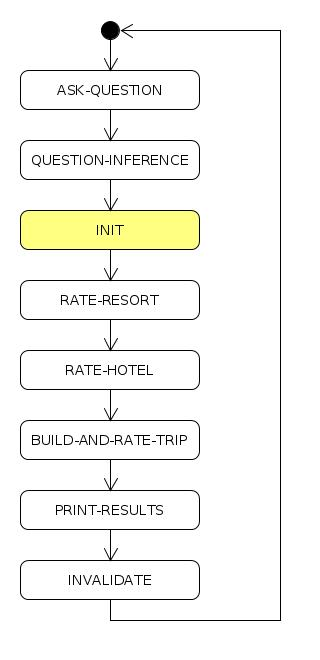
\includegraphics[width=0.4\textwidth]{loop}
  \caption{I moduli che compongono il loop principale del sistema esperto.}
  \label{loop}
\end{figure}

Il loop principale del sistema esperto, illustrato graficamente in figura \ref{loop}, si compone per la maggior parte di moduli di reasoning che sono pensati per operare in maniera ciclica. Di seguito si descrivono brevemente le funzioni svolte da ciascuno dei suddetti moduli.

\begin{itemize}
\item \textbf{ASK-QUESTION}\\
Pone all'utente una o più domande; le risposte vengono memorizzate per poi essere utilizzate dal modulo seguente.  Durante le iterazioni successive alla prima, ha inoltre il compito di chiedere all'utente se si ritiene soddisfatto da una delle soluzioni proposte al termine del ciclo precedente e, nel caso riceva risposta affermativa, arrestare l'esecuzione.
\item \textbf{QUESTION-INFERENCE}\\
Il modulo in esame si occupa di inferire le preferenze dell'utente a partire dalle riposte che egli fornisce. Ad esempio, se alla domanda ``Predilige località dal clima caldo o dal clima freddo?" l'utente risponde ``caldo", il sistema può dedurre che la tipologia di turismo più adatta in questo caso è ``balneare" associandogli un CF pari a $0.4$, mentre penalizzerà il turismo ``montano" associandogli un CF pari a $-0.4$.
\item \textbf{INIT}\\
Si occupa di eseguire alcune operazioni di inizializzazione, asserendo fatti che verranno utilizzati durante tutte le iterazioni successive. A differenza delle regole definite nei moduli seguenti, che vengono attivate ad ogni nuova iterazione, le regole del modulo \texttt{INIT} sono pensate per essere attivate un'unica volta in quanto legate a preferenze il cui grado di certezza non cambia nel tempo. In questa categoria ricadono ad esempio il numero di località che si desiderano visitare o la durata totale della villeggiatura. Alcune domande risultano essenziali per il corretto funzionamento del modulo \texttt{INIT} e pertanto il sistema non permette all'utente di ignorarle. 
\item \textbf{RATE-RESORT}\\
Contiene regole che vengono attivate ad ogni iterazione e hanno il compito di associare un ``punteggio" (in termini di CF) alle diverse località turistiche a partire dalle caratteristiche che le contraddistinguono e dalle preferenze espresse dall'utente.
\item \textbf{RATE-HOTEL}\\
Del tutto simile a \texttt{RATE-RESORT}, con la differenza che le regole riguardano gli hotel.
\item \textbf{BUILD-AND-RATE-TRIP}\\
Poiché i viaggi (trip) che ha senso creare e valutare cambiano di iterazione in iterazione, questo modulo ha il compito di generare suddette proposte di viaggio e valutarle sfruttando le informazioni create dai moduli precedenti. 
\item \textbf{PRINT-RESULTS}\\
I risultati ottenuti al termine della fase \texttt{BUILD-AND-RATE-TRIP} vengono presentati all'utente: un massimo di 5 proposte di viaggio sono quindi visualizzate in modo ordinato, partendo da quella che ha ottenuto la valutazione più alta. Per far sì che un viaggio venga preso in considerazione ed effettivamente proposto, il relativo CF deve essere maggiore di $0.35$. Nel caso in cui nessun viaggio superi suddetta soglia l'utente viene debitamente informato.
\item \textbf{INVALIDATE}\\
Il modulo ha il compito di rimuovere tutte quelle informazioni/valutazioni che devono essere ricalcolate all'iterazione successiva, la quale ha inizio non appena terminata la fase in esame.
\end{itemize}

\subsection{Organizzazione dei file}
L'organizzazione dei file riprende da vicino la suddivisione logica dei moduli. Sono infatti presenti due file, \texttt{domain.clp} e \texttt{reasoning.clp}, che contengono rispettivamente i moduli di dominio (principalmente definizioni di template e fatti) e i moduli di reasoning (esclusivamente regole).
Viene inoltre incluso un file che permette di avviare rapidamente il sistema esperto. È infatti sufficiente utilizzare il comando:
\begin{center}
\texttt{clips -f travel\_expert.clp}
\end{center}
per far sì che i file vengano caricati rispettando le dipendenze e l'esecuzione avviata.

\section{Template e scelte implementative}

La presente sezione analizza nel dettaglio alcuni dei template fondamentali per il funzionamento del sistema esperto realizzato, e allo stesso tempo tratta le scelte implementative correlate.

\subsection{Description-Value (DV)}

Il template più rilevante è di certo \texttt{dv}, definito all'interno del modulo \texttt{COMMON}. Tutte le informazioni a cui è associato un CF vengono rappresentate mediante questo template, il che permette di avere un unico insieme di regole per combinarli opportunamente.

\lstset{numbers=left,breaklines=true,language=C,basicstyle=\small\ttfamily}
\begin{lstlisting}[frame=single]
(deftemplate COMMON::dv 
    (slot dv-id (default-dynamic (gensym*)))
    (multislot description)
    (multislot value)
    (slot CF (type FLOAT) (range -1.0 1.0) (default 0.0))
    (slot basic (default FALSE)))   
\end{lstlisting}

A titolo di esempio si riportano anche alcune istanze del suddetto template, utili a comprendere l'uso che ne viene fatto: 

\begin{lstlisting}[frame=single]
(dv (dv-id gen3) (description the-tourism-type) (value mountain)
 (CF 0.4) (basic TRUE))
(dv (dv-id gen3) (description the-resort) (value Resort1)
 (CF 0.6) (basic FALSE))
(dv (dv-id gen15) (description the-hotel-in Resort1) (value Hotel3)
 (CF 0.3) (basic FALSE))
(dv (dv-id gen28) (description the-route) (value Resort1 Resort5) 
 (CF -0.2) (basic TRUE))
\end{lstlisting}

A questi fatti è possibile associare i seguenti significati: ``Il tipo di turismo ottimale è montano con CF 0.4", ``La località turistica ottimale è Resort1 con CF 0.6", ``Il miglior hotel nella località Resort1 è Hotel3 con CF 0.3" e infine ``L'utente percorre di buon grado la strada che connette Resort1 a Resort5 con CF -0.2". Come è possibile osservare, l'utilizzo di multislot sia per il campo descrizione che per il campo valore permette una notevole espressività e flessibilità.\\
Due fatti aventi stessa descrizione e stesso valore vengono combinati e il CF risultante è calcolato secondo regole precise: tali regole fanno anch'esse parte del modulo \texttt{COMMON} e godono di \texttt{auto-focus}, così da poter essere attivate in qualsiasi momento.\\
Lo slot \texttt{basic} permette di distinguere i fatti di base (dei quali si tiene ``memoria" tra un'iterazione e la successiva) dai fatti derivati (che al contrario vengono rimossi durante la fase \texttt{INVALIDATE}). Questa distinzione è necessaria in quanto i fatti \texttt{dv} derivati, poiché dipendono da altri fatti di tipo \texttt{dv}, devono essere ricalcolati ad ogni iterazione onde evitare comportamenti anomali. Per convincersene si consideri la seguente situazione:

\begin{enumerate}
\item Inizialmente, alla località Resort1 è associato un CF di $0.7$.
\item Una qualche regola stabilisce che la valutazione di un itinerario dipende dalla valutazione delle località che tocca. Durante la prima iterazione, pertanto, i cammini contenenti la località Resort1 saranno valutati tenendo conto del CF $0.7$ ad essa associato.
\item All'iterazione successiva l'utente esplicita una nuova preferenza, e a Resort1 viene associato un CF di $-0.2$. La regola per la combinazione dei fatti \texttt{dv} si attiva per prima e decrementa il CF di Resort1 portandolo a $0.625$.
\item A sua volta la regola per la valutazione degli itinerari si attiva, tenendo tuttavia conto del valore per Resort1 appena ottenuto dalla combinazione. Se la valutazione del cammino viene preservata tra una iterazione e la successiva, i cammini contenenti Resort1 di fatto verranno valutati una prima volta utilizzando il CF $0.7$ ed una seconda volta utilizzando il CF $0.625$. Poiché entrambi i CF risultano positivi, l'effetto finale è quello di valutare molto positivamente i path che contengono Resort1, cosa che in realtà non dovrebbe accadere. Ricalcolare da zero la valutazione del cammino (che è un'informazione derivata) tenendo conto solo del CF $0.625$ risolve questo problema.
\end{enumerate}
  
Infine, lo slot \texttt{dv-id} è incluso per poter eventualmente asserire più copie di uno stesso fatto un senza dover ricorrere alla duplicazione dei fatti in modo esplicito (usando cioè il comando \texttt{set-fact-duplication TRUE}).

\subsection{Resort e Hotel}

Di seguito vengono brevemente trattati i template relativi alle località ed agli hotel, che contengono le informazioni necessarie per buona parte del processo di rating.\\
Le qualità delle località, così come i collegamenti tra le stesse, non sono incluse direttamente nella definizione di \texttt{resort} bensì sono rappresentate sfruttando template dedicati. Ciò rende più agevole il pattern matching in diverse occasioni. \\
Per quanto riguarda gli hotel, è richiesto tener conto del flusso di turisti al fine di distribuirlo il più equamente possibile: anche questo aspetto è gestito tramite CF e rientra nei fattori considerati durante la valutazione degli hotel. Nello specifico, il rapporto tra posti letto disponibili e posti letto totali (\texttt{empty/capacity}) viene moltiplicato per una costante $c \in [0,1]$: quest'ultima può essere modificata a piacere per incrementare/decrementare l'influenza sul punteggio complessivo. Come prevedibile, si è osservato che un valore di $c$ troppo prossimo a 1 è da evitare in quanto tende a falsare la valutazione, ignorando le effettive preferenze dell'utente.
Infine, è possibile che \texttt{empty} risulti essere inferiore al numero di persone che partecipano al viaggio: in questo caso all'hotel viene associato un CF pari a $-1.0$ in modo da escluderlo automaticamente da qualsiasi proposta.

\begin{lstlisting}[frame=single]
(deftemplate RESORT::resort
    (slot name  (default ?NONE))
    (slot region (default ?NONE)))
  
(deftemplate RESORT::resort-tourism
    (slot resort-name  (default ?NONE))
    (slot tourism-type (default ?NONE))
    (slot score (type INTEGER) (range 1 5))) 
  
(deftemplate RESORT::route
    (slot resort-src (default ?NONE))
    (slot resort-dst (default ?NONE))
    (slot distance (type INTEGER) (range 1 ?VARIABLE)))
    
(deftemplate HOTEL::hotel
    (slot name (default ?NONE))
    (slot resort (default ?NONE))
    (slot stars (type INTEGER) (range 1 4))
    (slot empty (type INTEGER) (range 0 ?VARIABLE))
    (slot capacity (type INTEGER) (range 1 ?VARIABLE)))
\end{lstlisting} 

\subsection{Path, Duration e Trip}

Altri template che ricoprono un ruolo centrale sono \texttt{path}, \texttt{duration} e \texttt{trip}, definiti nel modulo \texttt{TRIP}:

\begin{lstlisting}[frame=single]
(deftemplate TRIP::path
    (slot path-id (default-dynamic (gensym*)))
    (multislot resorts)
    (slot length (type INTEGER))
    (slot total-distance (type INTEGER)))

(deftemplate TRIP::duration
    (multislot days (type INTEGER))
    (slot length (type INTEGER))
    (slot target (type INTEGER)))

(deftemplate TRIP::trip
    (slot trip-id (default-dynamic (gensym*)))
    (multislot resorts)
    (multislot hotels (default ND ND ND ND ND))
    (multislot days (type INTEGER))
    (multislot costs (type INTEGER) (default 0 0 0 0 0))
    (slot length (type INTEGER)))
\end{lstlisting}

I fatti che sono istanze di \texttt{path} e \texttt{duration} vengono asseriti una sola volta durante la fase \texttt{INIT} in quanto sia il numero di luoghi che l'utente intende visitare che la durata della vacanza non sono soggetti a raffinamenti successivi. Tali fatti vengono poi combinati tra loro in modo opportuno per generare, ad ogni iterazione, un certo numero di fatti di tipo \texttt{trip}.

Poiché l'utente non ha idea di quali mete visitare, si è optato per un approccio computazionalmente costoso ma in grado di fornire risultati interessanti. Inizialmente, viene creato un cammino (\texttt{path}) di lunghezza unitaria, che quindi comprende un'unica località. Dopo di che, i cammini vengono progressivamente prolungati di 1 considerando di volta in volta tutti i vicini dell'ultimo nodo inserito. Questo processo viene ripetuto fino a raggiungere la lunghezza desiderata o la massima lunghezza concessa. Per evitare di trattare un numero troppo elevato di combinazioni, è stata infatti limitata a 5 la lunghezza massima di qualsiasi cammino. Sempre per ragioni di complessità, vengono effettivamente considerati solo i path la cui lunghezza è esattamente quella richiesta e quelli che presentano una località in più/in meno. Tutti gli altri cammini vengono rimossi, anche perché si discosterebbero troppo dalle preferenze dell'utente. \\
Inoltre, lo slot \texttt{total-distance} è utilizzato per scartare i path che toccano le stesse località, ma che sono sub-ottimi in termini di distanze percorse: questo accorgimento non solo è utile ma è anche necessario, in quanto durante la valutazione dell'itinerario un cammino sub-ottimo può influire negativamente. Si consideri ad esempio il grafo riportato in figura \ref{graph}. Se si intendono toccare 4 località (nodi), molteplici cammini sono possibili, tra cui:

\begin{itemize}
\item il cammino ABCD, avente distanza totale $25 + 35 + 20 = 80$;
\item il cammino ABDC, avente distanza totale $25 + 15 + 20 = 60$;
\item il cammino ACDB, avente distanza totale $10 + 20 + 15 = 45$.
\end{itemize}

Assumendo che 20 sia la distanza massima che l'utente è disposto a percorrere per spostarsi da una località alla successiva, si può notare come la valutazione dell'itinerario è potenzialmente positiva, a patto che i nodi vengano visitati nell'ordine corretto. È quindi logico limitare la valutazione solo al path che risulta ottimale.\\
Un'ultima considerazione riguarda la scalabilità del metodo proposto. Verosimilmente, in presenza di un numero di località turistiche molto elevato, anche gli accorgimenti appena discussi non sarebbero sufficienti ad assicurare tempi di calcolo accettabili; un approccio alternativo potrebbe costringere l'utente a fornire una località/regione di partenza, e quindi limitarsi a calcolare solo gli itinerari che è possibile ottenere partendo da suddetta località/regione. \\

\begin{figure}[h]
  \centering
  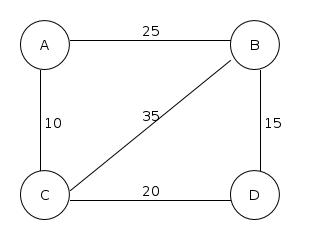
\includegraphics[width=0.5\textwidth]{graph}
  \caption{Un grafo di esempio, in cui ogni nodo rappresenta una località.}
  \label{graph}
\end{figure}

Anche nella costruzione dei fatti di tipo \texttt{duration} sono state fatte alcune assunzioni al fine di limitare la complessità del problema. Nelle considerazioni che seguono indicheremo con $G$ il numero di giorni di vacanza totali, con $L$ la lunghezza del cammino desiderata e con $(D_1, \dots, D_L)$ la ripartizione delle giornate in ciascuna delle località di un cammino. Nel caso in cui $G$ \texttt{mod} $L = 0$,  si assume che la soluzione ottimale sia porre $ D_i = G/L$  $\forall i$, ovvero trascorrere lo stesso numero di giorni in ogni località. In caso contrario si considerano solo quelle combinazioni tali che $| D_i - D_j | \leq K$ $(i \not = j , K \in \mathbb{N})$. Ad esempio, ponendo  $G = 15$, $L = 4$ e $ K = 1$ sono considerate valide le ripartizioni $(4, 4, 3, 4)$ e $(3, 4, 4, 4)$, ma non è valida la ripartizione $(5, 5, 2, 3)$. Lo scarto concesso può essere aumentato a piacere, al costo di una maggiore complessità computazionale dovuta all'aumento del numero di combinazioni ammissibili. \\

Combinando le informazioni relative a \texttt{path} e \texttt{duration} vengono infine generate le proposte di viaggio vere e proprie, ricorrendo alla regola di seguito riportata:

\begin{lstlisting}[frame=single]
(defrule BUILD-AND-RATE-TRIP::build-trip
    (iteration (number ?i))
    (path (path-id ?id) (resorts $?rs) (length ?len))
    (not (banned-path (path-id ?id)))
    (duration (days $?ds) (length ?len))
=>
    (assert (trip (resorts ?rs) (days ?ds) (length ?len))))
\end{lstlisting} 


Facendo riferimento alla linea 4, è possibile notare una condizione che contribuisce a restringere ulteriormente il campo di ricerca prima di procedere alla costruzione/valutazione dei viaggi. Infatti, solo quei path che non risultano ``bannati" vengono effettivamente utilizzati nella generazione delle proposte di viaggio. Un path viene considerato bannato se vale una delle seguenti condizioni:

\begin{enumerate}
\item il path include una località il cui CF è inferiore alla media dei CF di tutte le località;
\item il path contiene una località per la quale non esiste un hotel con un CF superiore ad una certa soglia minima (ad esempio $0.2$).
\end{enumerate}

Sono stati anche effettuati alcuni test con una versione alternativa della precedente definizione, la quale prevede che un path venga bannato solo quando almeno due delle località toccate soddisfano una delle condizioni sopra citate. Si è tuttavia osservato che la versione rilassata della regola causa un incremento del tempo di calcolo (in quanto più itinerari sono considerati validi e devono pertanto essere costruiti e valutati) senza fornire risultati significativamente migliori, ed è stata pertanto scartata. \\
Si noti che la condizione di ban per un path non è permanente, ma potenzialmente cambia ad ogni iterazione in seguito alla modifica dei CF di località ed hotel (il ban fa parte delle informazioni che vengono ritirate durante la fase \texttt{INVALIDATE}). \\
L'esecuzione procede con il rating dei fatti \texttt{trip} appena generati; tale valutazione tiene in considerazione diversi aspetti tra cui: località visitate, hotel in cui si pernotta, durata del soggiorno nelle diverse località e distanze fra le stesse, lunghezza del path, costo totale.

\section{Test e risultati ottenuti}

Durante lo sviluppo si è cercato di mantenere il codice più modulare possibile in modo da facilitare eventuali aggiornamenti futuri, un aspetto fondamentale per qualsiasi sistema esperto.
Attualmente il sistema è in grado di porre un totale di 23 domande, di cui buona parte può essere ignorata se l'utente lo desidera.
I test effettuati sono stati condotti predisponendo:
\begin{itemize}
\item 21 località turistiche, appartenenti a 2 regioni differenti;
\item una media di 2 hotel per ciascuna località turistica;
\item una media di 4 connessioni tra ciascuna località e quelle adiacenti.
\end{itemize}
Nelle condizioni attuali, ogni iterazione non impiega più di un paio di secondi per fornire un risultato. Le iterazioni successive alla prima, non dovendo ripetere la fase di \texttt{INIT} (che si occupa di compiti computazionalmente onerosi, come la costruzione dei path), spesso forniscono risposte pressoché istantanee.\\
Nella maggior parte delle situazioni gli itinerari proposti dal sistema risultano piuttosto coerenti con le richieste. Per quanto riguarda i casi in cui questo non accade, le cause sono spesso da ricercarsi in una effettiva carenza di soluzioni compatibili o in eventuali risposte contraddittorie da parte dell'utente (ad esempio ``voglio andare al mare e non in montagna; non amo i posti caldi, preferisco i posti freddi"). \\
Miglioramenti futuri potrebbero concentrarsi soprattutto sull'aggiunta di nuove domande, eventualmente anche molto specifiche, che guidino opportunamente il sistema nella sua ricerca. Inoltre, un'accurata operazione di ``fine-tuning" dei vari parametri utilizzati nella valutazione degli aspetti che caratterizzano un viaggio potrebbe portare a risultati ancora più apprezzabili.








